% --------- Body text  --------
\subsection{Data}
The modeling of the selected IS was carried out using a part of the data presented in Figure \ref{fig:immagine_larga}. Since not all of the fluxes of the sheet were included, in this subsection an explanation of the used data is provided. \\

\noindent Firstly, in \textbf{Veritas} (which integrates Ecoprogetto-Ricicli and MetalRecycling Venice), the incoming waste streams are chosen according to the final output of the three companies (see section 1.2). This means that only metal waste, glass waste, wood waste and mixed waste are included because the three companies produce only wood packaging, glass, and metal. This choice was made because considering other types of waste (such as plastic) would misrepresent the environmental benefit of the whole IS assessed later in the work. The waste is considered to be coming from the province of Venice and the municipality of Mogliano Veneto (TV), consequently from a community of approximately 890.000 people (Gruppo Veritas, n.d.).
Turning to Veritas's outgoing waste, two streams are recovered by being sent to the other two companies, meanwhile only the mixed waste coming out from MetalRecycling Venice was considered as <<waste to landfill>> 
\begin{equation*}
    w_{\text{Veritas,mix}}=\underset{\text{mixed waste}}{11410t} + \underset{\text{scraps}}{3536t} = 14946t
\end{equation*}
Secondly, in \textbf{Rilegno} the incoming waste is only wood, which comes in through two different flows: one from Veritas and another from other parts of Italy. The amount of wood given to Rilegno by the other regions in Italy was taken by the Annual Balance of Rilegno of 2019, and the amount of the incoming wood waste to Veritas was subtracted from that number. In 2019, Rilegno was able to recycle 63,8 \% of the recovered wood (Rilegno, 2019, p.36), which means that 36,2 \% went to landfill.
\begin{equation*}
    w_{\text{Rilegno,wood}}=x_{\text{Rilegno}}*36,2\%
\end{equation*}
Finally, in \textbf{Ecopatè} the only incoming waste is the selected glass provided by Veritas. This is the only company of the model that has an external input, which is still glass but coming from third parts.
Ecopatè's waste to landfill is considered as the sum of the glass scraps and other inerts given to R.I.V.E. S.r.l. which processes them to go to the landfill (see Figure \ref{fig:immagine_larga} for reference). Ecopatè also has some metal waste as a result of the glass treatment that is given back to Veritas to be recycled.
\begin{equation*}
    w_{\text{Ecopatè,glass}}=\underset{\text{inerts}}{14880 t} + \underset{\text{glass scraps}}{7290t}= 22800t 
\end{equation*}
\begin{equation*}
    w_{\text{Ecopatè,metal}}=\underset{\text{nonferrous metals}}{2160t}+\underset{\text{ferrous metals}}{6960t}=9120t
\end{equation*}
\vspace{3mm}

\noindent Table \ref{tab:wastetable} provides a representation of the waste distribution: in D the chosen fluxes coming from the 890.000 community are listed and in E the amount of wood waste coming from other parts of Italy is presented.
% ----- Table ----------
\begin{table*}[t]
\centering
\begin{tcolorbox}[
    colback=sapienza!5,     % Sfondo bordeaux chiarissimo
    colframe=sapienza!20,   % Bordo bordeaux tenue
    arc=3pt,                 % Smussatura degli angoli
    boxrule=1pt,             % Spessore del bordo
    width=\textwidth,        % Larghezza del box
    halign=center            % Centra il contenuto nel box
]
    \begin{tabular}{c | c c c c c | c}
    \toprule
    \textbf{Waste type} & \textbf{A} & \textbf{B} & \textbf{C} & \textbf{D} & \textbf{E} & \textbf{Total} \\
    \midrule \midrule 
    $w_{wood}$ & 0 & 0 & 1245353 t & 31800 t & 3408402 t  & 4685555 t \\
    \midrule
    $w_{glass}$ & 0 & 22800 t & 0 & 9000 t & 0 & 31800 t \\
    \midrule
    $w_{metal}$ & 0 & 9120 t & 0 & 44078 t  & 0 & 53198 t \\
    \midrule
    $w_{mix}$ & 14946 t & 0 & 0 & 135000 t & 0 & 149946 t \\
    \bottomrule
    \end{tabular}
\end{tcolorbox}

\vspace{5pt}
\caption{Tabular representation of the calculation of the waste vector}
\label{tab:wastetable}
\end{table*}
\newpage
\subsection{The Black Box method}
In figure \ref{fig:scheme}, the whole system is represented using the black box method, which treats each company as an entity that processes what comes in to get a product (output). The process always involves the production of some waste. The different flows are represented using arrows of specific colors, as explained in the legend. Each box is named by a letter displayed on the upper right side of the box, in order to show clearly the computation of the matrixes in the following part. 
\begin{center}
    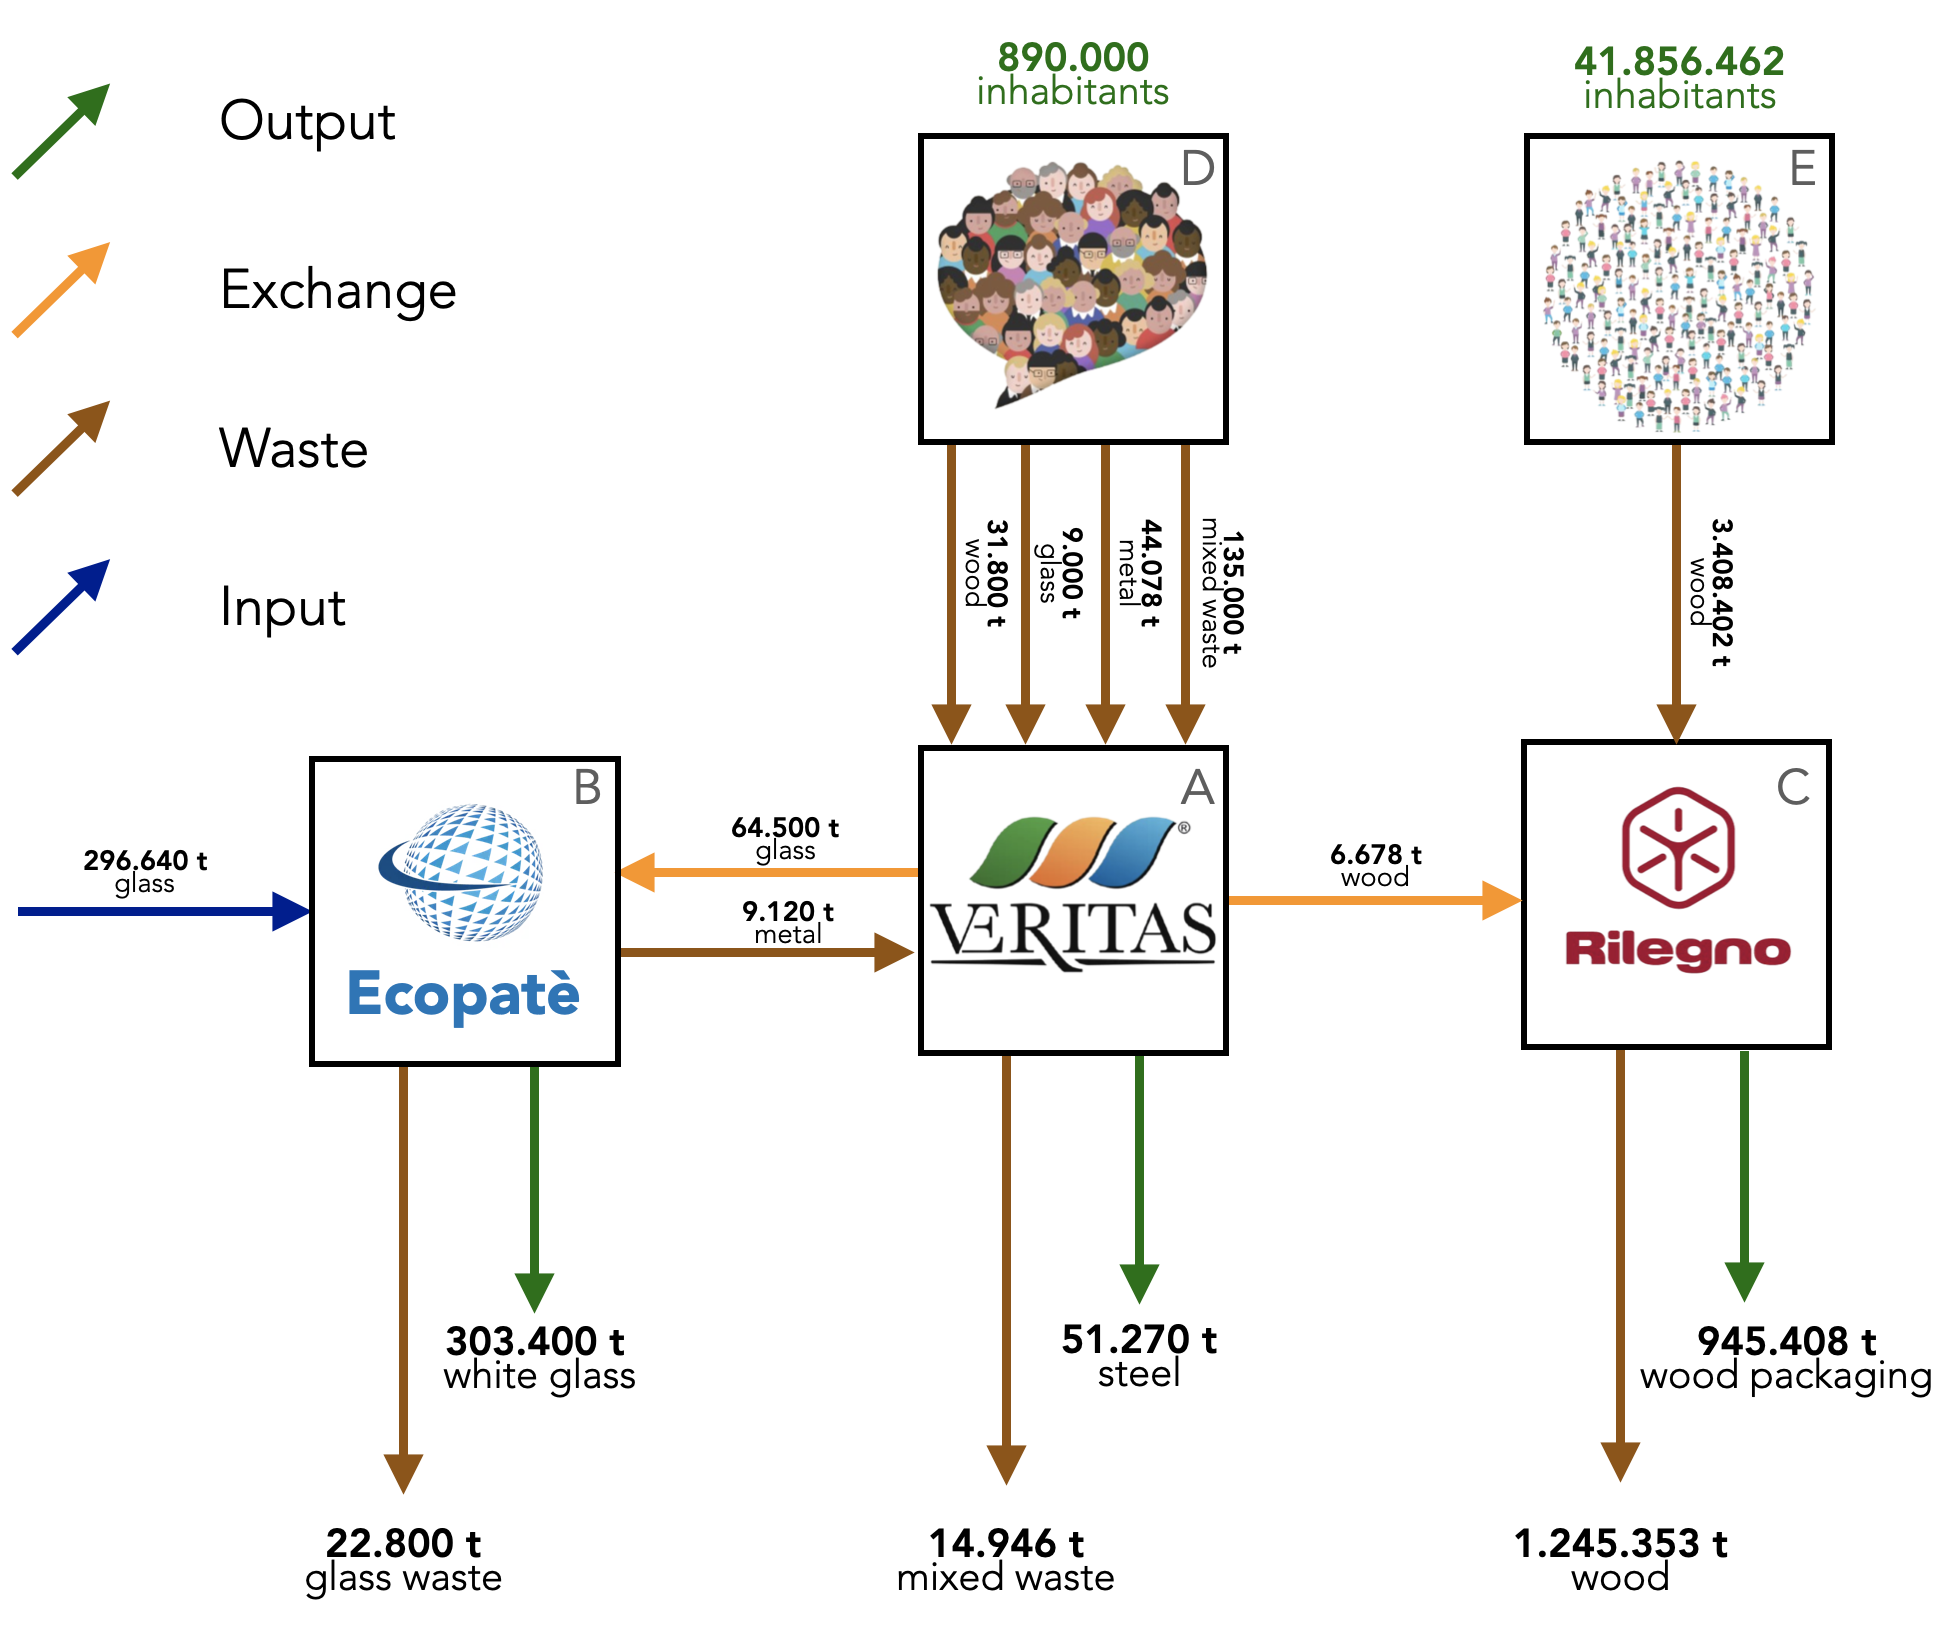
\includegraphics[width=0.95\linewidth]{schemapm.png}
    \captionof{figure}{Representation of the model through the black boxes method. Image created by the authors.}
    \label{fig:scheme}
\end{center}
As shown in figure \ref{fig:scheme}, to accurately map the IS, two additional boxes were included to represent the sources of waste and wood provided to Veritas and Rilegno, respectively. The group D represents the inhabitants of the Province of Venice and the municipality of Mogliano Veneto (TV) (Gruppo Veritas, n.d.) whereas group E considers the number of people that are served by Rilegno (Rilegno, 2019, p.14). 

%--input vector
\subsection{Vectors and Matrixes}
\subsubsection{Input vector}
The input vector shows the only present input of the system, that is the glass externally purchased by Ecopatè. Consequently, it is a vector with just one element.
        \begin{equation}
          \vec{r}=  
         \begin{bmatrix}
            r_{glass}
         \end{bmatrix}=
         \begin{bmatrix}
            296670
         \end{bmatrix}
        \end{equation}
        
 %--output vector
 \subsubsection{Output Vector}
 The output vector of the Ecodistretto di Porto Marghera considers the final outputs of each black box of the system. It is important to note that the output for boxes D and E is the number of inhabitants served by the respective company (Gruppo Veritas, n.d.) (Rilegno, 2019, p.14).
        \begin{equation}
            \vec{x}=
            \begin{bmatrix}
                x_{\text{Veritas}}\\
                x_{\text{Ecopatè}}\\
                x_{\text{Rilegno}}\\
                x_{\text{C.Veritas}}\\
                x_{\text{C.Rilegno}}\\
            \end{bmatrix}
            =
            \begin{bmatrix}
                51270 \\
                303400 \\
                945408 \\
                890000 \\
                41856462 \\
            \end{bmatrix}
        \end{equation}

%--waste vector
\subsubsection{Waste vector}
The waste vector regroups the different types of waste that appear in the system. Each element of the vector is the sum of all the specific waste that appears in the system. For more information on how the calculation is carried out, see Table \ref{tab:wastetable}.
        \begin{equation}
            \vec{w}=
            \begin{bmatrix}
                w_{wood} \\
                w_{glass} \\
                w_{metal} \\
                w_{mix}
            \end{bmatrix}
            =
            \begin{bmatrix}
                4685555 \\
                31800 \\
                53198 \\
                149946 
            \end{bmatrix}
        \end{equation}

 %-- Input matrix
 \subsubsection{Input matrix}
 The input matrix shows the distribution of each input among the different companies. In this case, the fact that there is only one input in the entire system implies that the matrix has only one row. Furthermore, each element of the matrix is calculated by dividing the input of the considered enterprise by its own output. The formula for each element of the matrix is the following one: 
 \begin{equation}
     r_{glass,j}=\frac{r_{glass}}{x_j}
 \end{equation}
 which leads to the input matrix for this case: 
 \begin{equation}
     R=
     \begin{bmatrix}
         0 & 0,98 & 0 & 0 & 0
     \end{bmatrix}
 \end{equation}
 
 %-- Waste matrix
 \subsubsection{Waste matrix}
  The waste matrix represents the distribution of each type of waste among the different companies of the model. Each element of the matrix is obtained using the formula (6):
 \begin{equation}
     w_{ij}=\frac{w_i}{x_j} \\
 \end{equation}
 where $w_i$ is the type of waste (wood, glass, etc.) and $x_j$ is the considered company (Veritas, ..., C.Rilegno).
\begin{equation}
    \label{eq:matrice_rifiuti}
    W = 
        \begin{blockarray}{cccccc}
        % Intestazioni di colonna
         & \text{A} & \text{B} & \text{C} & \text{D} & \text{E} \\
        \begin{block}{l[ccccc]}
        % Righe con etichetta laterale e contenuto
    w_{\text{wood}}  & 0    & 0 & 1,32 & 0,4  & 0,08 \\
    w_{\text{glass}} & 0    & 0 & 0    & 0,01 & 0    \\
    w_{\text{metal}} & 0    & 0 & 0    & 0    & 0    \\
    w_{\text{mix}}   & 0,29 & 0 & 0    & 0,15 & 0    \\
         \end{block}
         \end{blockarray}
\end{equation}

 %-- Z matrix
 \subsubsection{Z matrix}
 Finally, the Z matrix quantifies the exchanges between companies in tons. It specifies the participants and the amounts exchanged, reflecting only the two transactions depicted in Figure \ref{fig:scheme}.
 \begin{equation}
    \label{eq:matrice_z}
    Z = 
        \begin{blockarray}{cccccc}
        % Intestazioni di colonna
         & \text{A} & \text{B} & \text{C} & \text{D} & \text{E} \\
        \begin{block}{l[ccccc]}
        % Righe con etichetta laterale e contenuto
    A  & 0    & 64500 & 6678 & 0  & 0 \\
    B  & 0    & 0      & 0     & 0  & 0 \\
    C  & 0    & 0      & 0     & 0  & 0 \\
    D  & 0    & 0      & 0     & 0  & 0 \\
    E  & 0    & 0      & 0     & 0  & 0 \\
         \end{block}
         \end{blockarray}
\end{equation}